\documentclass{article}
\usepackage{amsmath}
\usepackage{pgfmath}
\usepackage{amssymb}
\usepackage{amsthm}
\usepackage{tikz}
\usepackage[a4paper, margin=0.8in]{geometry}
\usepackage{algorithm}
\usepackage{algpseudocode}
\usepackage{graphicx}
\usepackage{subcaption}
\usetikzlibrary{calc}
\usepackage{float}
\usepackage{caption}

\setlength{\parskip}{1em}
\setlength{\parindent}{0em}

\title{Case Analysis}
\author{Mohammed Rizin \\ Unemployed}

\date{\today}

\newcommand{\drawArray}[2]{%
    \newcount\arrayLength
    \begin{figure}[H]
        \centering
        \begin{tikzpicture}
            \coordinate (s) at (0, 0);
            \def\found{0}
            \arrayLength=0
            \foreach \num [count=\i from 0] in {#1} {
                \node[rectangle, draw, minimum size=6mm] at (s) {\num};
                \ifnum\num=#2
                    \node at ($(s)-(0,0.8)$) {$\underbrace{\i}_{key}$};
                    \xdef\found{1}
                \else
                    \node at ($(s)-(0,0.5)$) {\i};
                \fi
                
                \coordinate (s) at ($(s) + (0.6, 0)$);
                \ifnum\found=0
                \global\advance\arrayLength by 1
                \fi
            }
            \ifnum\found=0
                \node at ($0.45*(s) + (0, -1.0)$) {Not Found!};
            \fi
        \end{tikzpicture}
        \caption{Searching for key = #2 after \the\arrayLength \text{ steps}}
    \end{figure}
}

\begin{document}
\maketitle

\section{Linear Search Algorithm}

\newcommand{\A}{8, 6, 12, 5, 9, 7, 4, 3, 16, 18}

\begin{algorithm}
    \caption{Linear Search Algorithm}
    \label{linear_search}
    \begin{algorithmic}[1]
        \Procedure{LinearSearch}{$A, n, x$}
        \For {$i \gets 0$ to $n-1$}
        \If {$A[i] = x$}
        \State Return $i$
        \EndIf
        \EndFor
        \State Return $-1$
        \EndProcedure
    \end{algorithmic}
\end{algorithm}

\subsection{Best, Worst, Average Time}
Suppose we have an array:

\expandafter\drawArray\expandafter{\A}{3}
\expandafter\drawArray\expandafter{\A}{0}

Best Case $ B(n) \Longrightarrow$ Searching key element is present at index 0.  Then it will take $O(1)$. \\
Worst Case $ W(n) \Longrightarrow$ Either the element is absent or its at last index. Then it will take $O(n)$. \\
Average Case  $\Longrightarrow \frac{\text{all possible cases time}}{\text{no. of cases}}$\\
\\
Most of the cases, finding the average case time is not possible. But most of the cases it would be equal to Worst case time.

To calculate :
\[
\begin{aligned}
    Avg Time &= \frac{\sum_{i = 0}^{n} \text{time taken to find $i^{th}$ index element}}{n}\\
    AvgTime &= \frac{1+2+3+\cdots+n}{n}\\
    AvgTime &= \frac{\frac{n{(n+1)}}{2}}{n}\\
    AvgTime &= \frac{(n+1)}{2} \simeq O(n) \cong W(n)
\end{aligned}
\]

All these complexities are based on comparison operations you are doing. In average case, we considered every single possibility and then took the mean of it.

\subsection{Asymptotic Notations for Linear Search}
As mentioned earlier, Cases are no where related to notations. Notations apply to functions. But cases are related to Analysis of that function. 
\[
\begin{aligned}
B(n) &= 1\\
B(n) &= O(n)\\
B(n) &= \Omega(n)\\
B(n) &= \Theta(n)
\end{aligned}
\]

\[
\begin{aligned}
W(n) &= n\\
W(n) &= O(n)\\
W(n) &= \Omega(n)\\
W(n) &= \Theta(n)
\end{aligned}
\]

Don't get confused with $O(n)$ is for worst case scenario and $\Omega(n)$ is for best case scenario.

\section{Binary Search Tree}

\begin{figure}[H]
    \centering
    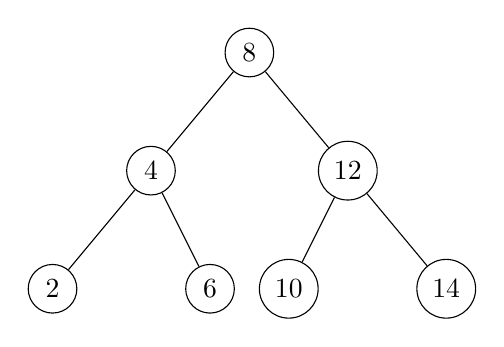
\begin{tikzpicture}[level distance=1.5cm, sibling distance=2.5cm]
        \node[circle, draw] {8}
            child {node[circle, draw] {4}
                child {node[circle, draw,] {2}}
                child {node[circle, draw, xshift=-0.5cm] {6}}
            }
            child {node[circle, draw] {12}
                child {node[circle, draw, xshift=+0.5cm] {10}}
                child {node[circle, draw, ] {14}}
            };

    \end{tikzpicture}
    \caption{Balanced Binary Search Tree: Minimum Heights}
\end{figure}

Binary Search Trees are used for searching. All the elements in the right is greater than element in the left.
If we are searching for smaller element, then we goto left hand side.

Suppose we are looking for element $2$:
We check if $2 \geq 8 ? No$, then go right.\\
We check if $2 \geq 4 ? No$, then go right.\\
if $2 \geq 2 ? Yes $, We found the element

Let us check how many comparison we have done. 
Generally the depth of a binary is $\log{n}$. So the number of comparisons are $\log{n}$ i.e. \boxed{O(\log{n})}.

\subsection{Analyze Best Case, Worst Case, Avg Case}
Best Case Time $B(n) \Longrightarrow $ Searching for the element at the root. This will take $O(1)$.
Worst Case Time $W(n) \Longrightarrow $ Searching for the element from below of the tree, i.e leaf. This will take $O(log{n})$, i.e. depends on the height of the tree.

We will not find $AvgTime$ in this case.
This is not the only binary search tree possible for the given elements.

\subsection{Skewed Binary Search Tree}
\begin{figure}[H]
    \centering
    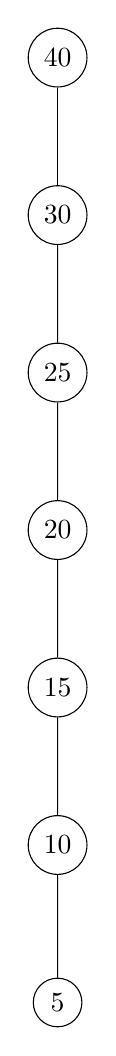
\begin{tikzpicture}[level distance=2.0cm, sibling distance=0.5cm]
        \node[circle, draw] {40}
        child {
            node[circle, draw] {30}
            child {
                node[circle, draw] {25}
                child {
                    node[circle, draw] {20}
                    child {
                        node[circle, draw] {15}
                        child {
                            node[circle, draw] {10}
                            child {
                                node[circle, draw] {5}
                            }
                        }
                    }
                }
            }
        };
    \end{tikzpicture}
    \caption{Left Skewed Binary Search Tree: Maximum height}
\end{figure}

\subsubsection{Analyze Best Case, Worst Case, Avg Case}
Best Case Time $B(n) \Longrightarrow $ Searching for the element at the root. This will take $O(1)$.
Worst Case Time $W(n) \Longrightarrow $ Searching for the element from below of the tree, i.e leaf. This will take $O(n)$, i.e. depends on the height of the tree.

\subsection{Conclusion: Binary Search Tree}
\boxed{
    \min{W(n)} = \log{n}\\
    } 
\boxed{
    \max{W(n)} = n\\
}

Worst case means maximum and its common to confuse how minimum of $\W(n)$. It depends on the type of tree or problem we are solving.

\end{document}